\subsection{Determining the Hole-Ice Parameters Corresponding to the Current Hole-Ice Approximation}
\label{sec:parameter_scan}

In current \clsim simulations that do not use the new medium-propagation
algorithm introduced by this study, an effective angular-acceptance
curve \(a\domhi(\eta)\) for optical modules is used to approximate the
effect of the hole ice on the detection of photons (section
\ref{sec:hole_ice_approximation}).

The hole-ice properties that have been assumed to create the effective
angular-acceptance curve \(a\domhi(\eta)\) are a hole-ice-cylinder
radius of \(30\cm\) and a geometric hole-ice scattering length of
\(\lambda\sca\hi = 50\cm\) (\textit{H2 model})
\cite{holeicestudieswithyag}. These properties can be used in a
\clsim simulation using the new medium-propagation algorithm and direct
propagation through the hole ice in order to compare the effective
angular-acceptance curve resulting from the simulation to the
approximation curve currently in use.

\docpar{This simulation using the H2 parameters is documented in \issue{80}.}

In the simulation, direct detection is used as acceptance criterion,
plane waves with an extend of \(e=1\m\) and a starting distance of
\(d=1\m\) are used. The hole-ice absorption length is set to a high
fixed value, \(\lambda\abs\hi = 100\m\). Figure \ref{fig:chie4Ite} shows
the result of this simulation. The angular-acceptance curve resulting
from the simulation does not match the approximation curve currently in
use very
well.\footnote{To make sure this is no matter of confusing effective scattering length and geometric scattering length, the same simulation has been performed with an effective scattering length of $50\cm$ rather than a geometric scattering length of $50\cm$. These curves match even worse. See appendix \ref{sec:angular_acceptance_simulation_for_h2_parameters}.}

\begin{figure}[htbp]
  \centering
  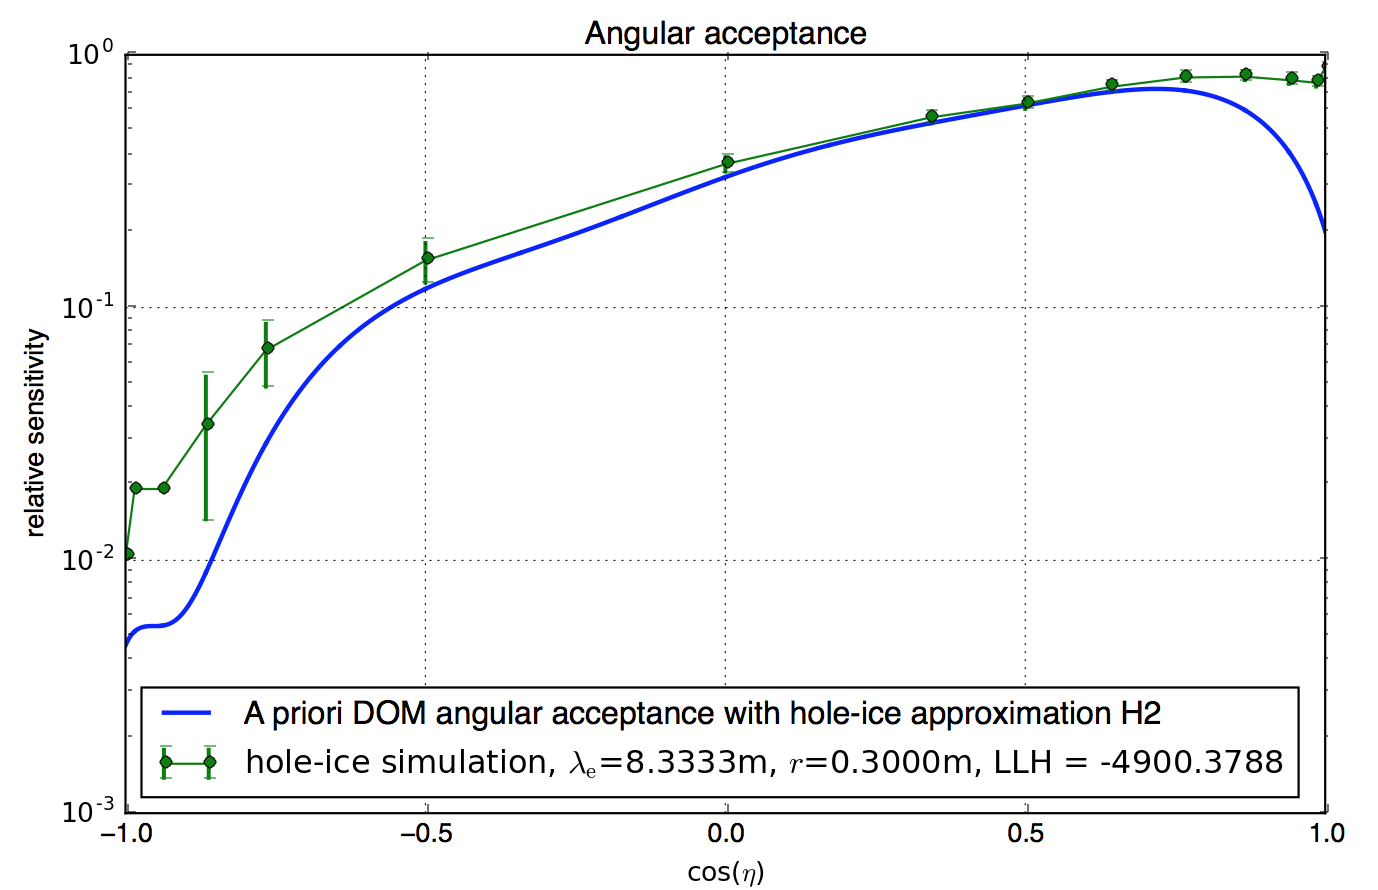
\includegraphics[width=0.75\textwidth]{img/angular-acceptance-karle-h2-vs-reference}
  \caption{Comparing the effective angular-acceptance curve currently in use for approximating the effect of hole ice on the detection of photons in simulations to a simulation with direct photon propagation through hole ice using the same hole-ice parameters, hole-ice-cylinder radius $r=30\cm$, geometric hole-ice scattering length $\lambda\sca\hi = 50\cm$. LLH is the log binomial likelihood comparing both curves.}
  \label{fig:chie4Ite}
\end{figure}

By performing a grid scan (see section
\ref{sec:cluster_parallelization}) over a range of hole-ice parameters,
one can find the best match with the approximation curve currently in
use, in order to understand which kind of direct-propagation hole ice
best matches the hole ice currently assumed in all simulations using the
approximation curve.

\docframe{
\docparwithoutframe{This grad scan is documented in \issue{12}.}\medskip

\sourceparwithoutframe{A script to configure and perform this kind of parameter scan is provided in \script{ParameterScan}.}
}

In principle, one could scan over a wide variety of parameters,
including the scattering and absorption lengths of the hole ice, the
hole-ice-cylinder radius, the distance from which the photons are
started towards the optical module, the kind of the photon source
(pencil beams, or plane waves), and the extent of the photon source
plane. In order to keep the computational effort minimal, however, all
conditions are kept the same as above, and only hole-ice-cylinder radius
and hole-ice scattering length are varied in the grid scan.

To compare the simulation results to the approximation curve, a binomial
likelihood \(L\) is used.

\begin{equation}
  L = \prod_{i=1}^N \binom{n}{k_i}\,p(\eta_i)^{k_i}\,(1-p(\eta_i))^{n-k_i}
\end{equation}

This likelihood can be interpreted as the probability that for a number
of \(N\) simulations, one simulation for each angle \(\eta_i\), starting
\(n\) photons from the angle \(\eta_i\) towards the optical module,
\(k_i\) photons will be accepted as hit by the optical module if the
acceptance probability \(p(\eta_i)\) for the angle \(\eta_i\) is given
by the approximation curve \(a\domhi(\eta)\),
\(p(\eta_i) = \sfrac{1}{g}\,a\domhi(\eta_i)\). \(g\) is a scaling factor
(see section \ref{sec:gauging}), which is needed due to the
normalization of \(a\domhi(\eta)\).

As one series of simulations is performed for each set \(\HH\) of
hole-ice parameters, there is a likelihood \(L_\HH\) for each parameter
set \(\HH\), which depends on the numbers \(k_{i,\HH}\) of photon hits
for photons started under the angle \(\eta_i\), propagated with hole-ice
parameters \(\HH\).

\[
  L_\HH = \prod_{i=1}^N \binom{n}{k_{i,\HH}}\,p(\eta_i)^{k_{i,\HH}}\,(1-p(\eta_i))^{n-k_{i,\HH}}
\]

The simulation resulting in the maximal likelihood \(L_\HHbest\)
corresponds to the set of hole-ice parameters \(\HHbest\) that best
describe the approximation curve \(a\domhi(\eta)\).

Figure \ref{fig:AWa5aiCh} shows the result of the parameter grid scan,
plotting the likelihood, or rather
\(-2\Delta\llh:= -2(\ln L_\HH - \ln L_\HHbest) = -2 \ln \left(\sfrac{L_\HH}{L_\HHbest}\right)\)
as a more common measure of agreement, against the effective scattering
length \(\lambda\esca\hi\) of the hole ice on the one axis, and the
radius \(r\) of the hole-ice cylinder on the other axis. For the optimal
parameters \(\HHbest\), \(\Delta\llh\) is zero.

\begin{figure}[htbp]
  \smallerimage{parameter-scan-contours}
  \caption{Agreement of the fixed hole-ice-approximation angular-acceptance curve $a\domhi(\eta)$ and direct hole-ice simulations using the new \clsim medium-propagation algorithm with hole-ice-cylinder radii $r$ given in units of the radius $r\dom$ of the optical module, and effective hole-ice scattering lengths $\lambda\esca\hi$. Each dot in the plot represents one parameter set $\HH$ and one corresponding set of simulations.}
  \label{fig:AWa5aiCh}
\end{figure}

The hole-ice parameters \(\HHbest\) that lead to a simulation, which
results in an angular-acceptance curve that best agrees with the
approximation curve \(a\domhi(\eta)\), are a hole-ice-cylinder radius
\(r = 1.0\,r\dom\) where \(r\dom\) is the radius of an optical module,
and an effective hole-ice scattering length \(\lambda\esca\hi = 1.3\m\).
Figure \ref{fig:weShir8i} shows an angular-acceptance curve for this
parameter set, as well as for the nearby parameter set of
\(r=1.0\,r\dom, \lambda\esca\hi = 1.0\m\).

\begin{figure}[htbp]
  \subcaptionbox{Simulation with hole-ice radius $r=1.0\,r\dom$ and effective hole-ice scattering length $\lambda\esca\hi = 1.3\m$.}{\halfimage{parameter-scan-best-angular}}\hfill
  \subcaptionbox{Simulation with hole-ice radius $r=1.0\,r\dom$ and effective hole-ice scattering length $\lambda\esca\hi = 1.0\m$.}{\halfimage{parameter-scan-1-1-angular}}
  \caption{Angular-acceptance curves from simulations best matching the hole-ice-approximation angular-acceptance curve $a\domhi(\eta)$. The LLH is the log binomial likelihood for the agreement of the simulation curve and the reference curve.}
  \label{fig:weShir8i}
\end{figure}

For photons approaching the optical module from below (right-hand side
of the plots), the simulations follow the approximation curve. For lower
angles, the simulation sees more photon hits, which, however, is the
case for all simulations in this grid scan.

To summarize this result, choosing a hole-ice cylinder of the same size
as the optical module, and an effective scattering length of about
\(1\m\) for a direct hole-ice simulation, comes closest to using the
hole-ice-approximation angular-acceptance curve, which is currently
default for \clsim simulations.
